\lecture{1}{mardi 04 février 2020}
\vspace{-1.2cm}

\section{Introduction au cours}

Qu'est-ce que l'ingénierie linguistique? Le nom de ce cours est ancien, aujourd'hui on dirait plutôt
"Introduction au Traitement Automatique des Langues (TAL)". On garde cet ancien nom car il est
intéressant (il mets en évidence qu'il s'agit d'un mix entre sciences "dures" et sciences "sociales"). \\

Il s'agit d'une discipline en constante évolution et hybride. Historiquement, deux disciplines dissociées et
ayant des chercheurs distincts existaient: d'un coté des linguistes s’interrogeant sur ce que l'informatique
pourrait apporter à leur discipline (linguistique informatique), et de l'autre des informaticiens et ingénieurs
curieux d'appliquer leurs modèles mathématiques dans l'étude de la linguistique (traitement automatique des langues).
À présent, les deux disciplines sont communes. \\

\textbf{Applications possibles de la discipline:}\\

\begin{minipage}[t]{0.5\textwidth}
\begin{itemize}
\item Correction orthographique/grammaticale
\item Traduction automatique/assistée
\item Reconnaissance et synthèse vocale
\end{itemize}
\end{minipage}
\begin{minipage}[t]{0.5\textwidth}
\begin{itemize}
\item Extraction d'informations
\item Analyse de sentiments
\item Question answering
\end{itemize}
\end{minipage}

\subsection{Niveaux linguistiques}

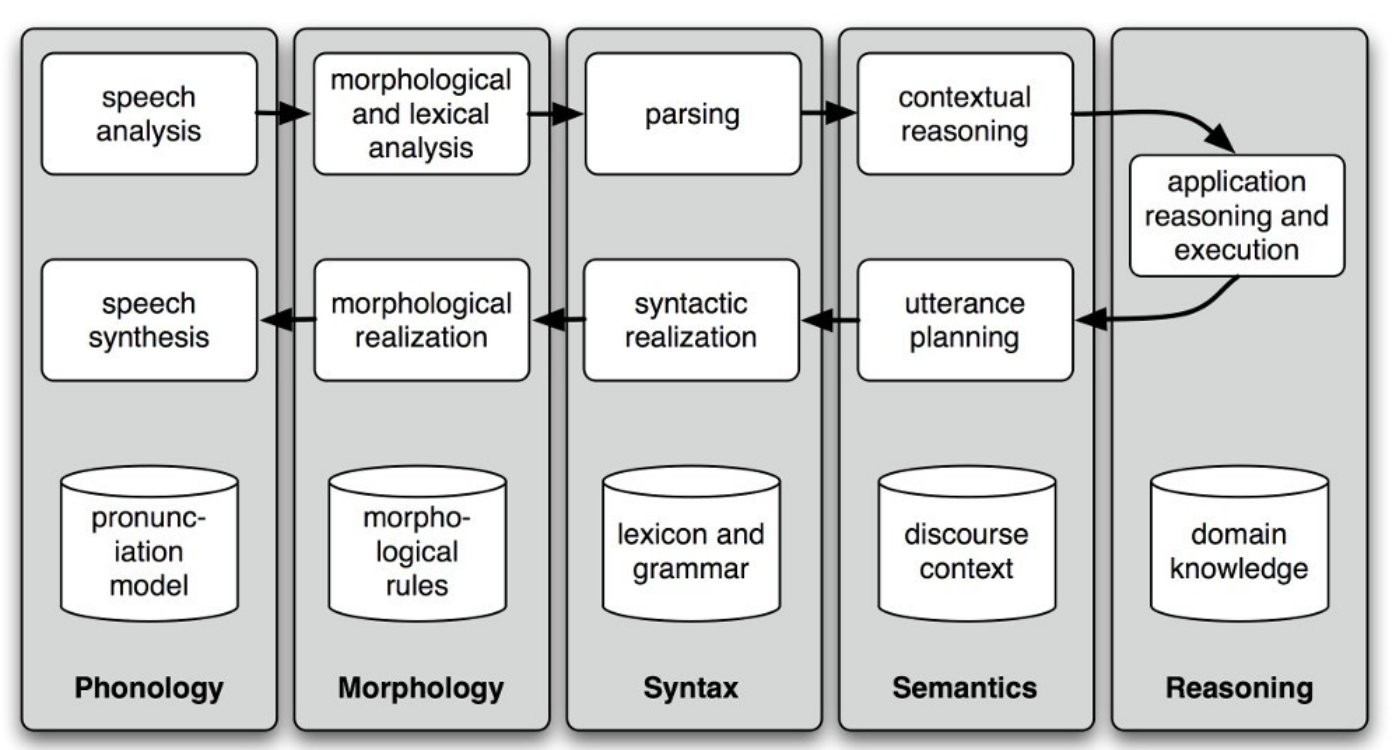
\includegraphics[scale=0.3]{lec1img1}\\ \\

Dans ce cours on étudie les nombreux niveaux linguistiques existants et les challenges qu'ils apportent au niveau
de l'ingénierie linguistique, car le langage humain est ambigu à tous les niveaux.\\

\begin{itemize}
    \item \textbf{Phonétique / Phonologie}: Hors scope du cours. Reconnaissance de mots depuis un signal audio et
    génération d'un signal audio à partir de mots. Prononciation, réalisation acoustique, etc.
    \item \textbf{Morphologie}: Reconnaissance des variations de forme des mots individuels (pluriel, conjugaison,...).
    \item \textbf{Lexique}: Qu'est-ce qu'un mot? Il faut savoir comment découper une phrase en mots pour la traiter par la suite.
    \item \textbf{Syntaxe}: Reconnaissance de l'ordre des mots et de l'organisation interne d'une phrase structurée.
    \item \textbf{Sémantique}: Reconnaissance du sens intrinsèque des mots (sémantique lexicale) ainsi que de la manière dont
    ils s'influencent mutuellement (sémantique compositionnelle).
    \item \textbf{Pragmatique}: Brièvement discuté lors du cours, mais hors scope du cours. Reconnaissance de l'intention du
    locuteur de la manière appropriée d'y répondre en fonction du contexte.
\end{itemize}

\subsection{Challenges affrontés}

\textbf{Ambigüités possibles:}

\begin{itemize}
    \item \textbf{Ambigüité phonétique}: Homophonie
    \item \textbf{Ambigüité morpho-lexicale}: Homographie
    \item \textbf{Ambigüité syntaxique}
    \item \textbf{Ambigüité sémantique}
    \item \textbf{Sémantique}: Hors contexte, certaines phrases peuvent être lues de façons différentes
    \item \textbf{Ambigüité pragmatique}: Ironie, par exemple
    \item \textbf{Ambigüité multilingue}
\end{itemize}

\noindent\textbf{Contraintes supplémentaires:}

\begin{itemize}
    \item \textbf{Précision}: Reproduire la compétence linguistique des êtres humains à l'aide de modèles
    formalisant notre compréhension
    \item \textbf{Rappel}: Une bonne couverture de la langue traitée requiert des ressources
    linguistiques (lexiques, grammaires,...) suffisamment fournies
    \item \textbf{Performance}: Un traitement rapide implique de limiter la complexité des modèles linguistiques
\end{itemize}

\subsection{Un peu d'histoire}

(TO DO)
